
\documentclass[20pt,landscape,a4paper,footrule]{foils}
\usepackage{solido-network-slides}
\usepackage{ulem}

% Basic things that we need are below
\selectlanguage{danish}

%\externaldocument{unix-audit-security-oevelser}
\externaldocument{\jobname-exercises}

\begin{document}
% beskrivelse findes i beskrivelse.txt

% lavet med basis i advanced-unix-admin kurset!

\mytitlepage
{IPv6 Security in Enterprise Networks}
{Marts 2012}


\hlkprofiluk


\slide{Planen idag}
\vskip 2 cm

\hlkimage{5cm}{dont-panic.png}
\centerline{\color{titlecolor}\LARGE Don't Panic!}

\begin{list1}
\item Kl 13:00-14:45
\item Mindre foredrag mere snak
\item Mindre enetale, mere foredrag 2.0 med socialt medie, informationsdeling og interaktion
\end{list1}
\centerline{Send gerne sp�rgsm�l senere}




\slide{Form�l: netv�rkssikkerhed for TCP/IP netv�rk}
\hlkimage{12cm}{1969_4-node_map.jpg}
\centerline{TCP/IP-baserede netv�rk - internet er overalt}

\slide{Form�l: mere specifikt}

\hlkimage{4cm}{IPv6ready.png}


\begin{list1}
\item At introducere TCP/IP version 6
\item Introducere specifikke sikkerhedsproblemer ved brug af IPv6
\end{list1}


\slide{Hackerv�rkt�jer}
% m�ske til reference afsnit?

\begin{list1}
\item Der benyttes en del v�rkt�jer:
\begin{list2}
\item Nmap, Nping - tester porte, godt til firewall admins \link{http://nmap.org}
\item Metasploit Framework gratis p� \link{http://www.metasploit.com/}
\item Wireshark avanceret netv�rkssniffer - \link{http://http://www.wireshark.org/} 
%\item Paros proxy \link{http://www.parosproxy.org}
\item Burpsuite \link{http://portswigger.net/burp/}
\item Skipfish \link{http://code.google.com/p/skipfish/}
\item Apache Tomcat J2EE servlet container \link{http://tomcat.apache.org}
\item OpenBSD operativsystem med fokus
  p� sikkerhed  \link{http://www.openbsd.org} 
\end{list2}
\end{list1}

\slide{BackTrack 5 og sniffer programmer}

\hlkimage{16cm}{bt5-revolution-blogpost-BTL.png}

\begin{list1}
\item Wireshark - \link{http://www.wireshark.org} avanceret netv�rkssniffer\\
bruger vi til at sniffe, vi bruger Wireshark til prim�re demo, n�vner Ettercap osv.
\item BackTrack \link{http://www.backtrack-linux.org/}
BackTrack er baseret p� Linux og m� kopieres frit :-)
\end{list1}



\slide{Status idag p� internet}

\hlkimage{18cm}{ipv4-address-report-2012.png}

Kilde: \link{http://www.potaroo.net/tools/ipv4/}


\slide{Why IPv6}

\hlkimage{5cm}{ipv4-run-out.png}
	

\slide{DDoS udviklingen, januar 2010 rapporten}

\hlkimage{15cm}{DDoS-2010.png}

Kilde:
\link{http://www.arbornetworks.com/report} 2009 rapporten



\slide{DDoS udviklingen, februar 2011}

\hlkimage{15cm}{ddos-2010-arbornetworks.png}

Kilde:
\link{http://www.arbornetworks.com/report} 2010 rapporten


\slide{Worldwide Infrastructure Security Report, 2010 Report}

\begin{quote}

{Key finding:\\
\bf Application-Layer DDoS Attacks Are Increasing in Sophistication and Operational Impact}\\
IDC and mobile/fixed wireless operators in particular are reporting significant outages, increased OPEX, customer churn and revenue loss due to application-layer DDoS attacks. These attacks are targeting both their customers and their own ancillary supporting services, such as DNS, Web portals, etc.\\
...\\
Conclusions\\
We further note that the fastest-growing category of ISPs-mobile and fixed wireless broadband operators-are also the least-prepared organizations in terms of network visibility, network control, and overall ability to successfully defend themselves and their customers against attack. These operators are balancing an overwhelming array of threats with conflicting budget pressures and business objectives.
\end{quote}

Mere komplekse trusler, betyder det flere firewall?


\slide{Worldwide Infrastructure Security Report 2010 Volume VI}

\begin{list2}
\item Application-Layer DDoS Attacks Are Increasing in Sophistication and Operational Impact
\item Mobile/Fixed Wireless Operators Are Facing Serious Challenges to Maintaining Availability in the Face of Attacks
\item Firewalls and IPS Devices Are Falling Short on DDoS Protection
\item DNS Has Broadly Emerged as an Attack Target and Enabler
\item {\bf Lack of Visibility into and Control over IPv6 Traffic Is a Significant Challenge}
\item Chronic Underfunding of Operational Security Teams
\item Operators Continue to Express Low Confidence in the Efficacy of Law Enforcement
\item Operators Have Little Confidence in Government Efforts to Protect Critical Infrastructure
\end{list2}

Kilde:
\link{http://www.arbornetworks.com/report} 


\slide{Worldwide Infrastructure Security Report 2011 Volume VII}

\begin{list2}
\item Ideologically-Motivated "Hactivism" and Vandalism Are the Most Readily-Identified DDoS Attack Motivations
\item 10 Gbps and Larger Flood-Based DDoS Attacks Are the "New Normal"
\item Increased Sophistication and Complexity of Application-Layer (Layer 7) DDoS Attacks and Multi-Vector DDoS Attacks Are Becoming More Common
\item Visibility and Security of Mobile and Fixed Wireless Networks Are an Ongoing Concern
\item {\bf First-Ever Reports of IPv6 DDoS Attacks "in the Wild" on Production Networks}
\item {\bf Rarity of IPv6-Enabled Attacks Indicates Low IPv6 Market Penetration and Lack of Critical Mass}
\item Stateful Firewalls, IPS and Load-Balancer Devices Continue to Fall Short on DDoS Protection Capabilities
\item The Overwhelming Majority of Network Operators Do Not Engage Law Enforcement 
\end{list2}

Kilde:
\link{http://www.arbornetworks.com/report} 



\slide{IPv6 is coming}

\hlkimage{2cm}{IPv6ready.png}

\begin{list1}
\item An important consideration is that IPv6 is quite likely to be already running on the enterprise network, whether that implementation was planned or not. Some important characteristics of IPv6 include:
\begin{list2}
\item IPv6 has a mechanism to automatically assign addresses so that end systems can easily establish communications.
\item IPv6 has several mechanisms available to ease the integration of the protocol into the network.
\item Automatic tunneling mechanisms can take advantage of the underlying IPv4 network and connect it to the IPv6 Internet.
\end{list2}
\end{list1}

Kilde:\\
{\footnotesize\link{http://www.cisco.com/en/US/prod/collateral/iosswrel/ps6537/ps6553/white_paper_c11-629391.html}}


\slide{Implications}

\hlkimage{2cm}{IPv6ready.png}

\begin{list1}
\item For an IPv4 enterprise network, the existence of an IPv6 overlay network has several of implications:
\begin{list2}
\item The IPv4 firewalls can be bypassed by the IPv6 traffic, and leave the security door wide open.
\item Intrusion detection mechanisms not expecting IPv6 traffic may be confused and allow intrusion
\item In some cases (for example, with the IPv6 transition technology known as 6to4), an internal PC can communicate directly with another internal PC and evade all intrusion protection and detection systems (IPS/IDS). Botnet command and control channels are known to use these kind of tunnels.
\end{list2}
\end{list1}

Kilde:\\
{\footnotesize\link{http://www.cisco.com/en/US/prod/collateral/iosswrel/ps6537/ps6553/white_paper_c11-629391.html}}


\slide{IPv6 in the Nordic region}

\hlkimage{14cm}{ipv6-nordic.png}

\link{http://v6asns.ripe.net/v/6?s=_ALL;s=DK;s=SE;s=NO;s=NL}

\slide{Metasploit IPv6}

\hlkimage{21cm}{metasploit-blog-ipv6.png}

Kilde:\\
{\small \link{https://community.rapid7.com/community/metasploit/blog/2012/03/07/}}



\slide{NIST Special Publication 800 series}

\hlkimage{16cm}{nist-sp-800-119.png}

\begin{list1}
\item SP 800-119	Dec. 2010	\emph{Guidelines for the Secure Deployment of IPv6}\\
God introduktion til IPv6 og sikkerhed i forbindelse med IPv6
\end{list1}

\link{http://csrc.nist.gov/publications/PubsSPs.html}



\slide{THC}

\begin{quote}
 A complete tool set to attack the inherent protocol weaknesses of IPV6
 and ICMP6, and includes an easy to use packet factory library.
\end{quote}


\begin{list1}

\item  Last update 2012-01-15 - opdateres l�bende\\
Current public version: v1.8 - CCC Camp release
\end{list1}


\link{http://thc.org/thc-ipv6/}


\slide{THC IPv6 [0x03] The Included Tools}

\begin{list2}
\item - parasite6: icmp neighbor solitication/advertisement spoofer, puts you
   as man-in-the-middle, same as ARP mitm (and parasite)
\item - alive6: an effective alive scanng, which will detect all systems
   listening to this address
\item - dnsdict6: parallized dns ipv6 dictionary bruteforcer
\item - fake\_router6: announce yourself as a router on the network, with the
  highest priority
\item - redir6: redirect traffic to you intelligently (man-in-the-middle) with
    a clever icmp6 redirect spoofer
\item - toobig6: mtu decreaser with the same intelligence as redir6
\item - detect-new-ip6: detect new ip6 devices which join the network, you can
    run a script to automatically scan these systems etc.
\item - dos-new-ip6: detect new ip6 devices and tell them that their chosen IP
    collides on the network (DOS).
\item - trace6: very fast traceroute6 with supports ICMP6 echo request and TCP-SYN
\item - flood\_router6: flood a target with random router advertisements
\item - flood\_advertise6: flood a target with random neighbor advertisements
\item - exploit6: known ipv6 vulnerabilities to test against a target
\item - denial6: a collection of denial-of-service tests againsts a target
\item - fuzz\_ip6: fuzzer for ipv6
\item - implementation6: performs various implementation checks on ipv6
\item - implementation6d: listen daemon for implementation6 to check behind a fw
\item - fake\_mld6: announce yourself in a multicast group of your choice on the net
\item - fake\_mld26: same but for MLDv2
\item - fake\_mldrouter6: fake MLD router messages
\item - fake\_mipv6: steal a mobile IP to yours if IPSEC is not needed for authentication
\item - fake\_advertiser6: announce yourself on the network
\item - smurf6: local smurfer
\item - rsmurf6: remote smurfer, known to work only against linux at the moment
\item - sendpees6: a tool by willdamn(ad)gmail.com, which generates a neighbor
          solicitation requests with a lot of CGAs (crypto stuff ;-) to keep the CPU busy. nice.
\item         - thcping6: sends a hand crafted ping6 packet
\item         [and about 15 more tools for you to discover]

\end{list2}


\slide{How to use IPv6}

\begin{center}
\vskip 3 cm
\hlkbig
www.solidonetworks.com

hlk@solidonetworks.com
\end{center}

\slide{Really how to use IPv6?}

\begin{list1}
\item Get IPv6 address and routing
\item Add AAAA (quad A) records to your DNS
\item Done
\end{list1}
\vskip 1cm
\centerline{\Large www.solidonetworks.com}

\begin{alltt}
\LARGE
www     IN	A       91.102.95.20
        IN	AAAA    2a02:9d0:10::9
\end{alltt}

\slide{IPv6 Status Denmark}

\begin{list1}
\item IT- og Telestyrelsen are becoming more active
\item Unofficial IPv6 task force at \link{http://www.ipv6tf.dk/}
\item Other initiatives \link{http://world-ipv6-day.dk/}
\item Major providers are ready on back bones
\item Internet Providers are increasingly becoming ready
\end{list1}



\slide{Collect information about IPv6}

\begin{list1}
\item \emph{Guidelines for the Secure Deployment of IPv6}, SP800-119, NIST\\
\link{http://csrc.nist.gov/publications/nistpubs/800-119/sp800-119.pdf}
\item \emph{The Second Internet: Reinventing Computer Networks with IPv6}, Lawrence E. Hughes, October 2010,\\ \link{http://www.secondinternet.org/}
\item \emph{IPv6 Network Administration}
af David Malone og Niall Richard Murphy
\item \link{http://www.ripe.net}
\item This presentation \smiley
\end{list1}

\slide{Allocating IPv6 addresses} 

\begin{list1}
\item You have plenty!
\item Providers and LIRs will typically get /32
\item Providers will typically give organisations /48 or /56
\item Your /48 can be used for:
\begin{list2}
\item 65536 subnets - all host subnets are /64
\item Each subnet has $2^{64}$ addresses
\end{list2}
\end{list1}

\slide{Preparing an IPv6
Addressing Plan}

\hlkimage{20cm}{ipv6-address-plan-ripe.png}

{\footnotesize \link{http://www.ripe.net/training/material/IPv6-for-LIRs-Training-Course/IPv6_addr_plan4.pdf}}

\slide{Example adress plan input}

\hlkimage{22cm}{ipv6-linked-to-ipv4.png}

\centerline{Easy and coupled with VLAN IDs it will work \smiley}

\slide{Run IPv6 in production}

\begin{list1}
\item Make sure you establish IPv6 in {\bf production}
\item Enabling service on IPv6 without production - bad experience for users
\item Start by enabling your DNS servers for IPv6 - and DNSSEC - and DNS over TCP\\
Remember that your firewall might have problems with large DNS packets
\item Add a production IPv6 router - hardware device or generic server
\item Tunnels are OK, and SixXS consider their service production
\end{list1}

\slide{IPv6 business case}


\begin{list2}
\item An almost unlimited scalability with a very large IPv6 address space ($2^128$ addresses), enabling IP addresses to each and every device.

\item Address self-configuration mechanisms, easing the deployment.

\item Improved security and authentication features, such as mandatory IPSec capacities and the possibility to use of the address space to include encryption keys.

\item Peer-to-peer connectivity, solving the NAT barrier with specific and permanent IP addresses for any device and/or user of the Internet.

\item Mobility features, enabling a seamless connexion when moving from one access point to another access point on the Internet.

\item Multi cast and any cast functionalities.

\item IPv6 will provide an easier remote interaction with each and every device with a {\bfseries direct integration to the Internet.} In other words, IPv6 will make possible to move from a network of servers, to a network of things.

\end{list2}

\centerline{ Business case for IPv6 is {\bf continuity}}


{\footnotesize Partial quote from http://www.smartipv6building.org/index.php/en/ipv6-potential}


\slide{IPv6: Internet redesigned? - no!}
 
\begin{list1}
\item Preserve the good stuff
\item back to basics, internet as it used to be!
\item fate sharing - connection rely on end points, not intermediary NAT boxes
\item end-to-end transparency - you have an address and I have an address
\item Wants: bandwidth +10G, low latency/predictable latency, Quality of Service, Security
\end{list1}

\vskip 5mm
\centerline{\color{titlecolor}\LARGE \bf IPv6 is evolution, not revolution}
\vskip 5mm

Note: IPv6 was not designed to solve all problems, so don't expect it to!


\slide{Up and running with IPv6}

\begin{list1}
%\item Join the fun - join the wireless network
\item Use ping/ping6 and traceroute to test connectivity
\item Try in your browser:
\begin{list2}
\item \link{http://www.kame.net} Dancing turtle
\item \link{http://www.ripe.net} RIPE, look for address up right corner 
\item \link{http://loopsofzen.co.uk/} Play a game
\item \link{https://www.sixxs.net/} Apply for IPv6 tunnel 
\end{list2}
\item Done \smiley
\end{list1}




% days 1-5
\slide{Dag 1 Basale begreber og mindre netv�rk}


\hlkimage{22cm}{images/kursus-netvaerk.pdf}


\slide{Netv�rk til routning}

\hlkimage{27cm}{basic-ipv6-network.pdf}

\vskip 2cm


\slide{Internet idag}


\hlkimage{12cm}{images/server-client.pdf}

\begin{list1}
\item Klienter og servere
\item R�dder i akademiske milj�er
\item Protokoller der er op til 20 �r gamle
\item Meget lidt kryptering, mest p� http til brug ved e-handel 
\item Kurset omhandler udelukkende netv�rk baseret p� IP protokollerne
\end{list1}

\slide{Internet er �bne standarder!}

{\hlkbig \color{titlecolor}
We reject kings, presidents, and voting.\\
We believe in rough consensus and running code.\\
-- The IETF credo Dave Clark, 1992.}

\begin{list1}
\item Request for comments - RFC - er en serie af dokumenter
\item RFC, BCP, FYI, informational\\
de f�rste stammer tilbage fra 1969
\item �ndres ikke, men f�r status Obsoleted n�r der udkommer en nyere
  version af en standard
\item Standards track:\\
Proposed Standard $\rightarrow$ Draft Standard $\rightarrow$ Standard
\item  �bne standarder = �benhed, ikke garanti for sikkerhed
\end{list1}


\slide{Hvad er Internet}

\begin{list1}
\item Kommunikation mellem mennesker!
\item Baseret p� TCP/IP
\begin{list2}
\item best effort
\item packet switching (IPv6 kalder det packets, ikke datagram)
\item forbindelsesorienteret, \emph{connection-oriented}
\item forbindelsesl�s, \emph{connection-less}
\end{list2}
\end{list1}

RFC-1958:
\begin{quote}
 A good analogy for the development of the Internet is that of
 constantly renewing the individual streets and buildings of a city,
 rather than razing the city and rebuilding it. The architectural
 principles therefore aim to provide a framework for creating
 cooperation and standards, as a small "spanning set" of rules that
 generates a large, varied and evolving space of technology.
\end{quote}


\slide{IP netv�rk: Internettet historisk set}

\begin{list2}  
\item[1961]  L. Kleinrock, MIT packet-switching teori
\item[1962]  J. C. R. Licklider, MIT - notes 
\item[1964]  Paul Baran: On Distributed Communications
\item[1969]  ARPANET startes 4 noder
\item[1971]  14 noder
\item[1973]  Arbejde med IP startes
\item[1973]  Email er ca. 75\% af ARPANET traffik
\item[1974]  TCP/IP: Cerf/Kahn: A protocol for Packet
        Network Interconnection
\item[1983]  EUUG $\rightarrow$ DKUUG/DIKU forbindelse
\item[1988]  ca. 60.000 systemer p� Internettet
        The Morris Worm rammer ca. 10\%
\item[2000]  Maj I LOVE YOU ormen rammer
%\item[2001]  August Code Red ~600.000 servere 
\item[2002]  Ialt ca. 130 millioner p� Internet
\end{list2}

\slide{Internet historisk set -  anno 1969}
\hlkimage{10cm}{1969_4-node_map.png}
%size 2

\begin{list2}
\item Node 1: University of California Los Angeles
\item Node 2: Stanford Research Institute
\item Node 3: University of California Santa Barbara
\item Node 4: University of Utah
%\item Kilde: \link{http://www.zakon.org/robert/internet/timeline/}
\end{list2}

\slide{De tidlige notater om Internet}

\begin{list1}
\item L. Kleinrock \emph{Information Flow in Large Communication nets}, 1961
\item J.C.R. Licklider, MIT noter fra 1962 \emph{On-Line Man Computer
  Communication} 
\item Paul Baran, 1964 \emph{On distributed Communications}
12-bind serie af rapporter\\
\link{http://www.rand.org/publications/RM/baran.list.html}
\item V. Cerf og R. Kahn, 1974 
\emph{A protocol for Packet Network Interconnection}
IEEE Transactions on Communication, vol. COM-22, pp. 637-648, May 1974
\item De tidlige notater kan findes p� nettet!
\end{list1}

L�s evt. mere i mit speciale \link{http://www.inet6.dk/thesis.pdf}

\slide{BSD UNIX}

\hlkimage{4cm}{implementation_freebsd.jpg}

\begin{list1}
  \item UNIX kildeteksten var nem at f� fat i for universiteter og
  mange andre
\item Bell Labs/AT\&T var et telefonselskab - ikke et software hus
\item P� Berkeley Universitetet blev der udviklet en del p� UNIX og
  det har givet anledning til en hel gren kaldet BSD UNIX
\item BSD st�r for Berkeley Software Distribution
\item BSD UNIX har blandt andet resulteret i virtual memory management
  og en masse TCP/IP relaterede applikationer
\end{list1}

\slide{Open Source definitioner - uddrag}

\begin{list1}
\item Free Redistribution - der m� ikke l�gges begr�nsninger p� om
  softwaren gives v�k eller s�lges
\item Source Code - kildeteksten skal v�re tilg�ngelig 
\item Derived Works - det skal v�re muligt at arbejde videre p� 
\item Integrity of The Author's Source Code - det skal v�re muligt at
  beskytte sit navn og rygte, ved at kr�ve �ndret navn for
  afledte projekter
\item Softwaren kaldes ofte ogs� Free Software, nogle bruger endda Libre
\item Eksempler er BSD licensen, Apache, GNU GPL og mange andre
\item Kilder: \link{http://www.opensource.org/}\\
\link{http://en.wikipedia.org/wiki/FLOSS} Free/Libre/Open-Source Software  
\end{list1}

\slide{BSD licensen er pragmatisk}

\begin{list1}
 \item BSD licensen kr�ver ikke at man offentligg�r sine �ndringer,
 man kan alts� bruge BSD kildetekst og stadig lave et kommercielt
 produkt!
\item GNU GPL bliver af nogle omtalt som en virus - der
  \emph{inficerer} softwaren, og afledte projekter
\end{list1}



\slide{Hvad er Internet}

\begin{list1}
\item 80'erne IP/TCP starten af 80'erne
\item 90'erne IP version 6 udarbejdes
  \begin{list2}
  \item IPv6 ikke brugt i Europa og US
  \item IPv6 er ekstremt vigtigt i Asien 
  \item historisk f� adresser tildelt til 3.verdenslande
  \item St�rre Universiteter i USA har ofte st�rre allokering end Kina!
  \end{list2}
\item 1991 WWW "opfindes" af Tim Berners-Lee hos CERN
\item E-mail var hovedparten af traffik
  - siden overtog web/http f�rstepladsen
\end{list1}

\slide{Hvad er Internet}

\vskip 1 cm

\centerline{Antallet af hosts p� Internet}

\hlkimage{16cm}{images/Count_Host.png}

\begin{list1}
\item Kilde: 
Hobbes' Internet Timeline v5.6\\
\link{http://www.zakon.org/robert/internet/timeline/}
\end{list1}

\slide{Hvad er Internet}

\vskip 1 cm

\centerline{Antallet af World Wide Web servere}

\hlkimage{16cm}{images/Count_WWW.png}  

\begin{list1}
\item Kilde: Hobbes' Internet Timeline v5.6\\
\link{http://www.zakon.org/robert/internet/timeline/}
\end{list1}


% IP-adresser

\slide{F�lles adresserum}

\vskip 2 cm
\hlkimage{17cm}{IP-address.pdf}

\begin{list1}
\item Hvad kendetegner internet idag
\item Der er et f�lles adresserum baseret p� 32-bit adresser
\item En IP-adresse kunne v�re 10.0.0.1
\end{list1}

\slide{IPv4 addresser og skrivem�de}

\begin{alltt}
hlk@bigfoot:hlk$ ipconvert.pl 127.0.0.1
Adressen er: 127.0.0.1
Adressen er: 2130706433
hlk@bigfoot:hlk$ ping 2130706433
PING 2130706433 (127.0.0.1): 56 data bytes
64 bytes from 127.0.0.1: icmp_seq=0 ttl=64 time=0.135 ms
64 bytes from 127.0.0.1: icmp_seq=1 ttl=64 time=0.144 ms
\end{alltt}

\begin{list1}
\item IP-adresser skrives typisk som decimaltal adskilt af punktum
\item Kaldes {\bf dot notation}: 10.1.2.3
\item Kan ogs� skrive som oktal eller heksadecimale tal
\end{list1}



\slide{IP-adresser som bits}

\begin{alltt}
IP-adresse: 127.0.0.1
Heltal:	2130706433
Binary:	1111111000000000000000000000001
\end{alltt}

\begin{list1}
\item IP-adresser kan ogs� konverteres til bits
\item Computeren regner bin�rt, vi bruger dot-notationen
\end{list1}

\slide{Internet ABC}

\begin{list1}
\item Tidligere benyttede man klasseinddelingen af IP-adresser: A, B, C, D og E
\item Desv�rre var denne opdeling ufleksibel:
\begin{list2}
\item A-klasse kunne potentielt indeholde 16 millioner hosts
\item B-klasse kunne potentielt indeholder omkring 65.000 hosts
\item C-klasse kunne indeholde omkring 250 hosts
\end{list2}
\item Derfor bad de fleste om adresser i B-klasser - s� de var ved at l�be t�r!
\item D-klasse benyttes til multicast
\item E-klasse er blot reserveret
\item Se evt. \link{http://en.wikipedia.org/wiki/Classful\_network}
\end{list1}


\slide{CIDR Classless Inter-Domain Routing}

\hlkimage{15cm}{CIDR-aggregation.pdf}

\begin{list1}
\item Subnetmasker var oprindeligt indforst�et
\item Dern�st var det noget man brugte til at opdele sit A, B eller C net med
\item Ved at tildele flere C-klasser kunne man spare de resterende B-klasser - men det bet�d en routing table explosion
\item Idag er subnetmaske en sammenh�ngende r�kke 1-bit der angiver st�rrelse p� nettet
\item 10.0.0.0/24 betyder netv�rket 10.0.0.0 med subnetmaske 255.255.255.0
\item Nogle f� steder kaldes det tillige supernet, supernetting
\end{list1}


\slide{Subnet calculator, CIDR calculator}

\hlkimage{10cm}{subnet-calculator.png}

\begin{list1}
\item Der findes et v�ld af programmer som kan hj�lpe med at udregne
subnetmasker til IPv4
\item Screenshot fra \link{http://www.subnet-calculator.com/}
\end{list1}


\slide{RFC-1918 private netv�rk}

\begin{list1}
\item Der findes et antal adresserum som alle m� benytte frit:
\begin{list2}
\item 10.0.0.0    -  10.255.255.255  (10/8 prefix)
\item 172.16.0.0  -  172.31.255.255  (172.16/12 prefix)
\item 192.168.0.0 -  192.168.255.255 (192.168/16 prefix)
\end{list2}
\item Address Allocation for Private Internets RFC-1918 adresserne!
\item NB: man m� ikke sende pakker ud p� internet med disse som afsender, giver ikke mening
\end{list1}

\slide{IPv4 addresser opsummering}

\begin{list2}
\item Altid 32-bit adresser
\item Skrives typisk med 4 decimaltal dot notation 10.1.2.3
\item Netv�rk angives med CIDR Classless Inter-Domain Routing RFC-1519
\item CIDR notation 10.0.0.0/8 -
  fremfor 10.0.0.0 med subnet maske 255.0.0.0
\item Specielle adresser\\
127.0.0.1 localhost/loopback\\
0.0.0.0  default route
\item RFC-1918 angiver private adresser som alle kan bruge

\end{list2}


\slide{Stop - netv�rket idag}

\begin{list1}
\item Bem�rk hvilket netv�rk vi bruger idag
\item Prim�re server fiona har IP-adressen 10.0.45.36
\item Prim�re router luffe har IP-adressen 10.0.45.2 (og flere andre)
\item Sekund�re router idag er Bianca som har IP-adressen 10.0.46.2 (og flere andre)  
\item Hvis du kender til IP i forvejen s� udforsk gerne p� egen h�nd netv�rket
\item Det er tilladt at logge ind p� alle systemer, undtagen Henrik's laptop bigfoot :-)
\item {\bf Det er forbudt at �ndre IP-konfiguration og passwords}
\item Nu burde I kunne forbinde jer til netv�rket fysisk, check med \verb+ping 10.0.45.2+
\item Det er nok at en PC i hver gruppe er p� kursusnetv�rket
\end{list1}

\centerline{Pause for dem hvor det virker, mens vi ordner resten}


\slide{OSI og Internet modellerne}

\hlkimage{14cm,angle=90}{images/compare-osi-ip.pdf}


\slide{Netv�rkshardware}

\begin{list1}
\item Der er mange muligheder med IP netv�rk, IP kr�ver meget lidt
\item Ofte benyttede idag er:
\begin{list2}
\item Ethernet - varianter 10mbit, 100mbit, gigabit, 10 Gigabit findes, men er dyrt
\item Wireless 802.11 teknologier
\item ADSL/ATM teknologier til WAN forbindelser
\item MPLS ligeledes til WAN forbindelser
\end{list2}
\item Ethernet kan bruge kobberledninger eller fiber
\item WAN forbindelser er typisk fiber p� grund af afstanden mellem routere
\item Tidligere benyttede inkluderer: X.25, modem, FDDI, ATM, Token-Ring
\end{list1}

\slide{Ethernet stik, kabler og dioder}

\hlkimage{20cm}{ethernetLights.jpg}

\centerline{Dioder viser typisk om der er link, hastighed samt aktivitet}

\slide{Tr�dl�se teknologier}

\hlkimage{10cm}{WCG200v2_med.jpg}

\begin{list1}
\item Et typisk 802.11 Access-Point (AP) der har Wireless og Ethernet stik/switch
\end{list1}

\slide{MAC adresser}
%\hlkimage{10cm}{apple-oui.png}

\begin{alltt}
00-03-93   (hex)        Apple Computer, Inc.
000393     (base 16)    Apple Computer, Inc.
                        20650 Valley Green Dr.
                        Cupertino CA 95014
                        UNITED STATES
\end{alltt}
\begin{list1}
\item Netv�rksteknologierne benytter adresser p� lag 2
\item Typisk svarende til 48-bit MAC adresser som kendes fra Ethernet MAC-48/EUI-48
\item F�rste halvdel af adresserne er Organizationally Unique Identifier (OUI)
\item Ved hj�lp af OUI kan man udlede hvilken producent der har produceret netkortet
\item \link{http://standards.ieee.org/regauth/oui/index.shtml}
\end{list1}

\slide{Half/full-duplex og speed}

\hlkimage{20cm}{half-full-duplex.pdf}

\begin{list1}
\item Hvad hastighed overf�res data med?
\item De fleste nyere Ethernet netkort kan k�re i fuld-duplex
\item med full-duplex kan der b�de sendes og modtages data samtidigt
\item Ethernet kan benytte auto-negotiation - der ofte virker\\
Klart bedre i gigabitnetkort men pas p�
\end{list1}





\slide{Broer og routere}

\hlkimage{20cm}{wan-network.pdf}
\centerline{Fysisk er der en begr�nsing for hvor lange ledningerne m� v�re}

\slide{Bridges}

\begin{list1}
\item Ethernet er broadcast teknologi, hvor data sendes ud p� et delt medie - �teren
\item Broadcast giver en gr�nse for udbredningen vs hastighed
\item Ved hj�lp af en bro kan man forbinde to netv�rkssegmenter p� layer-2
\item Broen kopierer data mellem de to segmenter
\item Virker som en forst�rker p� signalet, men mere intelligent
\item Den intelligente bro kender MAC adresserne p� hver side
\item Broen kopierer kun hvis afsender og modtager er p� hver sin side
\end{list1}

Kilde: For mere information s�g efter Aloha-net\\ \link{http://en.wikipedia.org/wiki/ALOHAnet}


\slide{En switch}

\hlkimage{15cm}{switch-1.pdf}

\begin{list1}
\item Ved at forts�tte udviklingen kunne man samle broer til en switch
\item En switch idag kan sende og modtage p� flere porte samtidig, og med full-duplex
\item Bem�rk performance begr�nses af backplane i switchen
\end{list1}

\slide{Topologier og Spanning Tree Protocol}

\hlkimage{18cm}{switch-STP.pdf}

Se mere i bogen af Radia Perlman, \emph{Interconnections: Bridges, Routers, Switches, and Internetworking Protocols}


\slide{Core, Distribution og Access net}

\hlkimage{20cm}{core-dist.pdf}

\centerline{Det er ikke altid man har pr�cis denne opdeling, men den er ofte brugt}




\slide{Pakker i en datastr�m}

\hlkimage{23cm}{ethernet-frame-1.pdf}
\begin{list1}
\item Ser vi data som en datastr�m er pakkerne blot et m�nster lagt henover data 
\item Netv�rksteknologien definerer start og slut p� en frame
\item Fra et lavere niveau modtager vi en pakke, eksempelvis 1500-bytes fra Ethernet driver
\end{list1}



\slide{IPv4 pakken - header - RFC-791}

\begin{alltt}
\small  
    0                   1                   2                   3   
    0 1 2 3 4 5 6 7 8 9 0 1 2 3 4 5 6 7 8 9 0 1 2 3 4 5 6 7 8 9 0 1 
   +-+-+-+-+-+-+-+-+-+-+-+-+-+-+-+-+-+-+-+-+-+-+-+-+-+-+-+-+-+-+-+-+
   |Version|  IHL  |Type of Service|          Total Length         |
   +-+-+-+-+-+-+-+-+-+-+-+-+-+-+-+-+-+-+-+-+-+-+-+-+-+-+-+-+-+-+-+-+
   |         Identification        |Flags|      Fragment Offset    |
   +-+-+-+-+-+-+-+-+-+-+-+-+-+-+-+-+-+-+-+-+-+-+-+-+-+-+-+-+-+-+-+-+
   |  Time to Live |    Protocol   |         Header Checksum       |
   +-+-+-+-+-+-+-+-+-+-+-+-+-+-+-+-+-+-+-+-+-+-+-+-+-+-+-+-+-+-+-+-+
   |                       Source Address                          |
   +-+-+-+-+-+-+-+-+-+-+-+-+-+-+-+-+-+-+-+-+-+-+-+-+-+-+-+-+-+-+-+-+
   |                    Destination Address                        |
   +-+-+-+-+-+-+-+-+-+-+-+-+-+-+-+-+-+-+-+-+-+-+-+-+-+-+-+-+-+-+-+-+
   |                    Options                    |    Padding    |
   +-+-+-+-+-+-+-+-+-+-+-+-+-+-+-+-+-+-+-+-+-+-+-+-+-+-+-+-+-+-+-+-+

                    Example Internet Datagram Header
\end{alltt}


\slide{IP karakteristik}

\begin{list1}
\item F�lles adresserum
\item Best effort - kommer en pakke fra er det fint, hvis ikke m� h�jere lag klare det
\item Kr�ver ikke mange services fra underliggende teknologi \emph{dumt netv�rk}
\item Defineret gennem �ben standardiseringsprocess og RFC-dokumenter
\end{list1}



\slide{Fragmentering og PMTU}

\hlkimage{20cm}{fragments-1.pdf}
\begin{list1}
\item Hidtil har vi antaget at der blev brugt Ethernet med pakkest�rrelse p� 1500 bytes
\item Pakkest�rrelsen kaldes MTU Maximum Transmission Unit 
\item Skal der sendes mere data opdeles i pakker af denne st�rrelse, fra afsender
\item Men hvad hvis en router p� vejen ikke bruger 1500 bytes, men kun 1000
\end{list1}

\slide{ICMP Internet Control Message Protocol}

\begin{list1}
\item Kontrolprotokol og fejlmeldinger
\item Nogle af de mest almindelige beskedtyper
\begin{list2}
\item echo
\item netmask
\item info
\end{list2}
\item Bruges generelt til \emph{signalering}
\item Defineret i RFC-792
\end{list1}

\centerline{\bf NB: nogle firewall-administratorer blokerer alt ICMP - det er forkert!}

\slide{ICMP beskedtyper}

\begin{list1}
\item Type
\begin{list2}
\item 0 = net unreachable;
\item 1 = host unreachable;
\item 2 = protocol unreachable;
\item 3 = port unreachable;
\item 4 = fragmentation needed and DF set;
\item 5 = source route failed.
\end{list2}
\item Ved at fjerne ALT ICMP fra et net fjerner man n�dvendig funktionalitet!
\item Tillad ICMP types:
\begin{list2}
\item 3 Destination Unreachable
\item 4 Source Quench Message
\item 11 Time Exceeded
\item 12 Parameter Problem Message
\end{list2}
\end{list1}

\slide{Hvordan virker ARP?}

\begin{center}
\colorbox{white}{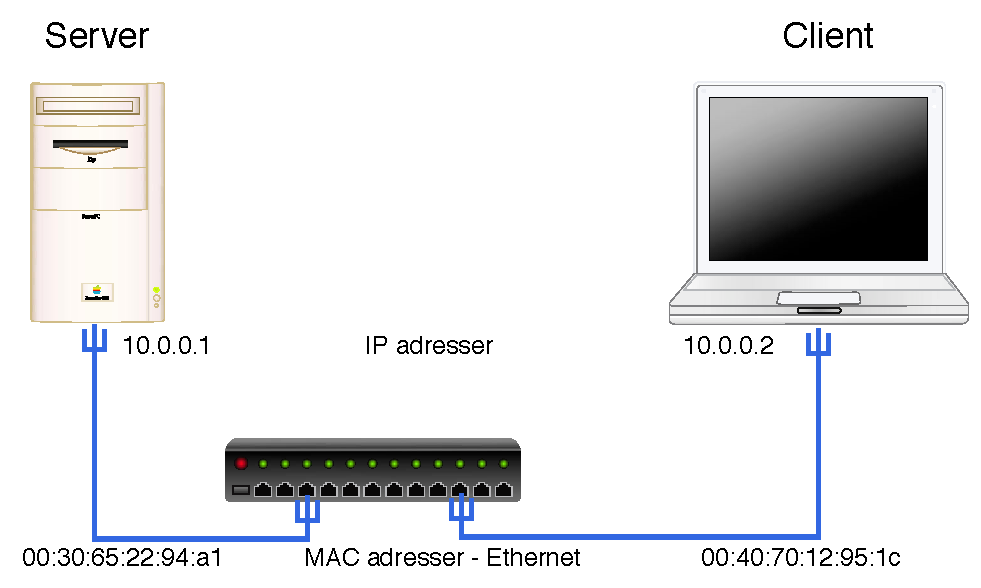
\includegraphics[width=18cm]{images/arp-basic.pdf}}  
\end{center}

%server 00:30:65:22:94:a1\\
%client 00:40:70:12:95:1c\\
%hacker 00:02:03:04:05:06\\

\slide{Hvordan virker ARP? - 2}
\begin{list1}
\item {\bfseries ping 10.0.0.2} udf�rt p� server medf�rer
\item ARP Address Resolution Protocol request/reply:
  \begin{list2}
  \item ARP request i broadcast - Who has 10.0.0.2 Tell 10.0.0.1
  \item ARP reply (fra 10.0.0.2) 10.0.0.2 is at 00:40:70:12:95:1c
  \end{list2}
\item IP ICMP request/reply:
  \begin{list2}
    \item Echo (ping) request fra 10.0.0.1 til 10.0.0.2
\item Echo (ping) reply fra 10.0.0.2 til 10.0.0.1
\item ...
  \end{list2}
\item ARP udf�res altid p� Ethernet f�r der kan sendes IP trafik
\item (kan v�re RARP til udstyr der henter en adresse ved boot)
\end{list1}


\slide{ARP cache}

\begin{alltt}
\small
hlk@bigfoot:hlk$ arp -an        
? (10.0.42.1) at 0:0:24:c8:b2:4c on en1 [ethernet]
? (10.0.42.2) at 0:c0:b7:6c:19:b on en1 [ethernet]
\end{alltt}

\begin{list1}
\item ARP cache kan vises med kommandoen \verb+arp -an+
\item -a viser alle
\item -n viser kun adresserne, pr�ver ikke at sl� navne op - typisk hurtigere
\item ARP cache er dynamisk og adresser fjernes automatisk efter 5-20 minutter hvis de ikke bruges mere
\item L�s mere med \verb+man 4 arp+
\end{list1}


\slide{Manualsystemet}

\begin{quote}
 It is a book about a Spanish guy called Manual. You should read it.
       -- Dilbert
\end{quote}

\begin{list1}
\item Manualsystemet i UNIX er utroligt st�rkt!
\item Det SKAL altid installeres sammen med v�rkt�jerne!
\item Det er n�sten identisk p� diverse UNIX varianter!  
\item \verb+man -k+ s�ger efter keyword, se ogs� \verb+apropos+
\end{list1}

Pr�v \verb+man crontab+ og \verb+man 5 crontab+

\hlkimage{10cm}{images/unix-command-1.pdf}

\slide{En manualside}

\begin{alltt}
\small
CAL(1)                BSD General Commands Manual                CAL(1)
NAME
     cal - displays a calendar
SYNOPSIS
     cal [-jy] [[month]  year]
DESCRIPTION
   cal displays a simple calendar.  If arguments are not specified, the cur-
   rent month is displayed.  The options are as follows:
   -j      Display julian dates (days one-based, numbered from January 1).
   -y      Display a calendar for the current year.

The Gregorian Reformation is assumed to have occurred in 1752 on the 3rd
of September.  By this time, most countries had recognized the reforma-
tion (although a few did not recognize it until the early 1900's.)  Ten
days following that date were eliminated by the reformation, so the cal-
endar for that month is a bit unusual.

HISTORY
     A cal command appeared in Version 6 AT&T UNIX.  
\end{alltt}

\slide{Kommandolinien p� UNIX}

\begin{list1}
\item Shells kommandofortolkere:
  \begin{list2}
    \item sh - Bourne Shell
\item bash - Bourne Again Shell
\item ksh - Korn shell, lavet af David Korn
\item csh - C shell, syntaks der minder om C sproget
\item flere andre, zsh, tcsh 
  \end{list2}
\item Svarer til command.com og cmd.exe p� Windows
\item Kan bruges som komplette programmeringssprog
\end{list1}

\slide{Kommandoprompten}


\begin{alltt}    
\small
[hlk@fischer hlk]$ id
uid=6000(hlk) gid=20(staff) groups=20(staff), 
0(wheel), 80(admin), 160(cvs) 
[hlk@fischer hlk]$ 

[root@fischer hlk]# id
uid=0(root) gid=0(wheel) groups=0(wheel), 1(daemon),
2(kmem), 3(sys), 4(tty), 5(operator), 20(staff), 
31(guest), 80(admin) 
[root@fischer hlk]#
\end{alltt}

\begin{list1}  
\item typisk viser et dollartegn at man er logget ind som almindelig bruge
\item mens en havel�ge at man er root - superbruger
\end{list1}

\slide{Kommandoliniens opbygning}


\begin{alltt}
echo [-n] [string ...]  
\end{alltt}

\begin{list1}
\item Kommandoerne der skrives p� kommandolinien skrives s�dan:
\begin{list2}
\item Starter altid med kommandoen, man kan ikke skrive \verb+henrik echo+
\item Options skrives typisk med bindestreg foran, eksempelvis \verb+-n+
\item Flere options kan s�ttes sammen, \verb+tar -cvf+ eller \verb+tar cvf+
\item I manualsystemet kan man se valgfrie options i firkantede
  klammer \verb+[]+
\item Argumenterne til kommandoen skrives typisk til sidst (eller der
  bruges redirection)
\end{list2}
\end{list1}


\slide{Adgang til UNIX}

\begin{center}

\includegraphics[width=4cm]{images/kde.png}

\includegraphics[width=4cm]{images/gnome-logo-large.png}
\end{center}

\begin{list1}
%\item Systemer der minder om UNIX kan idag nemt skaffes
\item Adgang til UNIX kan ske via grafiske brugergr�nseflader
  \begin{list2}
%  \item X11 \link{http://www.x.org}
  \item KDE \link{http://www.kde.org}
  \item GNOME \link{http://www.gnome.org}
  \end{list2}
\item eller kommandolinien
\end{list1}
\centerline{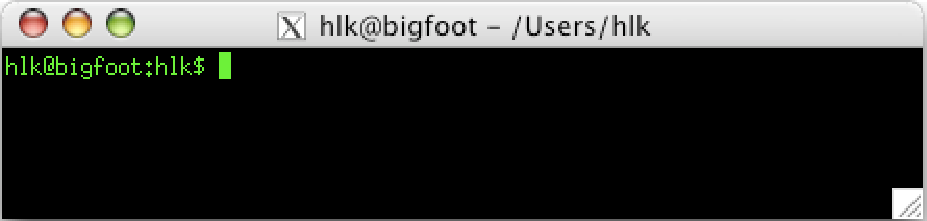
\includegraphics[width=17cm]{images/unix-cmdline.pdf}}


\exercise{ex:putty-install}


\exercise{ex:winscp-install}

\exercise{ex:unix-login}

\exercise{ex:unix-cal}

\exercise{ex:sudo}



\exercise{ex:unix-boot-cd}




\exercise{ex:unix-basic-commands}



\slide{TCP/IP basiskonfiguration}

\begin{alltt}
ifconfig en0 10.0.42.1 netmask 255.255.255.0
route add default gw 10.0.42.1 
\end{alltt}

\begin{list1}
\item konfiguration af interfaces og netv�rk p� UNIX foreg�r med:
\item \verb+ifconfig+, \verb+route+ og \verb+netstat+  
\item - ofte pakket ind i konfigurationsmenuer m.v.
\item fejls�gning foreg�r typisk med \verb+ping+ og \verb+traceroute+
\item P� Microsoft Windows benyttes ikke \verb+ifconfig+\\
men kommandoerne \verb+ipconfig+ og \verb+ipv6+
\end{list1}


\slide{Sm� forskelle}

\begin{alltt}
$ route add default 10.0.42.1
\emph{uden gw keyword!}

$ route add default gw 10.0.42.1 
\emph{Linux kr�ver gw med}
\end{alltt}

\vskip 1cm

\centerline{\bf NB: UNIX varianter kan indbyrdes v�re forskellige!}



\slide{Flere sm� forskelle}

\vskip 1cm 
\centerline{ping eller ping6}

\begin{list1}
\item Nogle systemer v�lger at ping kommandoen kan ping'e b�de IPv4 og Ipv6
\item Andre v�lger at \verb+ping+ kun benyttes til IPv4, mens IPv6 ping kaldes for \verb+ping6+
\item L�g ogs� m�rke til jargonen \emph{at pinge}
\end{list1}


\slide{OpenBSD}

Netv�rkskonfiguration p� OpenBSD:
\begin{alltt}
# cat /etc/hostname.sk0
inet 10.0.0.23 0xffffff00 NONE
# cat /etc/mygate
10.0.0.1
# cat /etc/resolv.conf    
domain security6.net
lookup file bind
nameserver 212.242.40.3
nameserver 212.242.40.51
\end{alltt}

\slide{FreeBSD}

Netv�rkskonfiguration p� FreeBSD \verb+/etc/rc.conf+:
\begin{alltt}
\small
# This file now contains just the overrides from /etc/defaults/rc.conf.
hostname="freebsd.security6.net
#ifconfig_vr0="DHCP"
ifconfig_vr0="inet 10.20.30.75 netmask 255.255.255.0"
router_enable="NO"
defaultrouter="10.20.30.65"
keyrate="fast"
moused_enable="YES"
ntpdate_enable="NO"
ntpdate_flags="none"
saver="blank"
sshd_enable="YES"
usbd_enable="YES"
...
\end{alltt}


\slide{GUI v�rkt�jer - autoconfiguration}

\hlkimage{20cm}{osx-network-automatic.png}

\slide{GUI v�rkt�jer - manuel konfiguration}

\hlkimage{20cm}{osx-network-manual.png}

\slide{ifconfig output}

\begin{alltt}\small
hlk@bigfoot:hlk$ ifconfig -a
lo0: flags=8049<UP,LOOPBACK,RUNNING,MULTICAST> mtu 16384
        inet 127.0.0.1 netmask 0xff000000 
        inet6 ::1 prefixlen 128 
        inet6 fe80::1%lo0 prefixlen 64 scopeid 0x1 
gif0: flags=8010<POINTOPOINT,MULTICAST> mtu 1280
stf0: flags=0<> mtu 1280
en0: flags=8863<UP,BROADCAST,SMART,RUNNING,SIMPLEX,MULTICAST> mtu 1500
        ether 00:0a:95:db:c8:b0 
        media: autoselect (none) status: inactive
        supported media: none autoselect 10baseT/UTP <half-duplex> 10baseT/UTP <full-duplex> 10baseT/UTP <full-duplex,hw-loopback> 100baseTX <half-duplex> 100baseTX <full-duplex> 100baseTX <full-duplex,hw-loopback> 1000baseT <full-duplex> 1000baseT <full-duplex,hw-loopback> 1000baseT <full-duplex,flow-control> 1000baseT <full-duplex,flow-control,hw-loopback>
en1: flags=8863<UP,BROADCAST,SMART,RUNNING,SIMPLEX,MULTICAST> mtu 1500
        ether 00:0d:93:86:7c:3f 
        media: autoselect (<unknown type>) status: inactive
        supported media: autoselect
\end{alltt}
%$
\vskip 1 cm
\centerline{ifconfig output er n�sten ens p� tv�rs af UNIX}




\slide{Vigtigste protokoller}


\begin{list1}
\item ARP Address Resolution Protocol
\item IP og ICMP Internet Control Message Protocol
\item UDP User Datagram Protocol
\item TCP Transmission Control Protocol
\item DHCP Dynamic Host Configuration Protocol 
\item DNS Domain Name System
\end{list1}
\vskip 1cm
\centerline{Ovenst�ende er omtrent minimumskrav for at komme p� internet}

% allerede gennemg�et ovenfor
%\slide{ICMP}

%\begin{list1}
%\item 	Internet Control Message Protocol 
%	Defineret i RFC-792

%\end{list1}


\slide{UDP User Datagram Protocol}
\hlkimage{20cm}{udp-1.pdf}
\begin{list1}
\item Forbindelsesl�s RFC-768, \emph{connection-less} - der kan tabes pakker
\item Kan benyttes til multicast/broadcast - flere modtagere
\end{list1}



\slide{TCP Transmission Control Protocol}
\hlkimage{20cm}{tcp-1.pdf}

\begin{list1}
\item Forbindelsesorienteret RFC-791 September 1981, \emph{connection-oriented}
\item Enten overf�res data eller man f�r fejlmeddelelse
\end{list1}




\slide{TCP three way handshake}

\hlkimage{7cm}{images/tcp-three-way.pdf}

\begin{list2}
\item {\bfseries TCP SYN half-open} scans
\item Tidligere loggede systemer kun n�r der var etableret en fuld TCP
  forbindelse - dette kan/kunne udnyttes til \emph{stealth}-scans
\item Hvis en maskine modtager mange SYN pakker kan dette fylde
  tabellen over connections op - og derved afholde nye forbindelser
  fra at blive oprette - {\bfseries SYN-flooding}
\end{list2}

\slide{Well-known port numbers}

\hlkimage{10cm}{iana1.jpg}

\begin{list1}
\item IANA vedligeholder en liste over magiske konstanter i IP
\item De har lister med hvilke protokoller har hvilke protokol ID m.v.
\item En liste af interesse er port numre, hvor et par eksempler er:
\begin{list2}
\item Port 25 SMTP Simple Mail Transfer Protocol
\item Port 53 DNS Domain Name System
\item Port 80 HTTP Hyper Text Transfer Protocol over TLS/SSL
\item Port 443 HTTP over TLS/SSL
\end{list2}
\item Se flere p� \link{http://www.iana.org}
\end{list1}

\slide{Hierarkisk routing}

\hlkimage{18cm}{routing-1.pdf}
Hvordan kommer pakkerne frem til modtageren

\slide{IP default gateway}

\hlkimage{13cm}{routing-2.pdf}

\begin{list1}
\item IP routing er nemt
\item En host kender en default gateway i n�rheden
\item En router har en eller flere upstream routere, f� adresser den sender videre til
\item Core internet har default free zone, kender \emph{alle netv�rk} 
\end{list1}



\slide{DHCP Dynamic Host Configuration Protocol}

\hlkimage{13cm}{dhcp-1.pdf}

\begin{list1}
\item Hvordan f�r man information om default gateway
\item Man sender et DHCP request og modtager et svar fra en DHCP server
\item Dynamisk konfiguration af klienter fra en centralt konfigureret server
\item Bruges til IP adresser og meget mere
\end{list1}


\slide{Routing}


\begin{list1}
  \item routing table - tabel over netv�rkskort og tilh�rende adresser
\item default gateway - den adresse hvortil man sender
  \emph{non-local} pakker\\kaldes ogs� default route, gateway of last
  resort
\item routing styres enten manuelt - opdatering af route tabellen,
  eller konfiguration af adresser og subnet maske p� netkort
\item eller automatisk ved brug af routing protocols - interne og
  eksterne route protokoller
\item de lidt �ldre routing protokoller har ingen sikkerhedsmekanismer
\item {\bf IP benytter longest match i routing tabeller!}
\item Den mest specifikke route g�lder for forward af en pakke!
\end{list1}


\slide{Routing forst�else}

\begin{alltt}
\small
$ netstat -rn
Routing tables

Internet:
Destination    Gateway         Flags  Refs      Use  Netif 
default        10.0.0.1        UGSc    23        7    en0
10/24          link#4          UCS      1        0    en0
10.0.0.1       0:0:24:c1:58:ac UHLW    24       18    en0  
10.0.0.33      127.0.0.1       UHS      0        1    lo0
10.0.0.63      127.0.0.1       UHS      0        0    lo0
127            127.0.0.1       UCS      0        0    lo0
127.0.0.1      127.0.0.1       UH       4     7581    lo0
169.254        link#4          UCS      0        0    en0  
\end{alltt}

\vskip 1 cm
\centerline{Start med kun at se p� Destination, Gateway og Netinterface}


\exercise{ex:network-ifconfig}
\exercise{ex:network-netstat}
\exercise{ex:network-lsof}


\slide{whois systemet}

\begin{list1}
\item IP adresserne administreres i dagligdagen af et antal Internet
  registries, hvor de st�rste er:
\begin{list2}
\item RIPE (R�seaux IP Europ�ens)  \link{http://ripe.net}
\item ARIN American Registry for Internet Numbers \link{http://www.arin.net}
\item Asia Pacific Network Information Center \link{http://www.apnic.net}
\item LACNIC (Regional Latin-American and Caribbean IP Address Registry) - Latin America and some Caribbean Islands
\end{list2}
\item disse fire kaldes for Regional Internet Registries (RIRs) i
  mods�tning til Local Internet Registries (LIRs) og National Internet
  Registry (NIR) 
\end{list1}

\slide{whois systemet-2}

\begin{list1}
\item ansvaret for Internet IP adresser ligger hos ICANN The Internet
  Corporation for Assigned Names and Numbers\\
\link{http://www.icann.org}
\item NB: ICANN m� ikke forveksles med IANA Internet Assigned Numbers
  Authority \link{http://www.iana.org/} som bestyrer portnumre m.v.
\end{list1}

\exercise{ex:whois}


% basic ping og traceroute

\slide{Ping}

\begin{list1}
\item ICMP - Internet Control Message Protocol
\item Benyttes til fejlbeskeder og til diagnosticering af forbindelser
\item ping programmet virker ved hj�lp af ICMP ECHO request og
  forventer ICMP ECHO reply
\item 
\begin{alltt}
\small {\bfseries 
$ ping 192.168.1.1}
PING 192.168.1.1 (192.168.1.1): 56 data bytes
64 bytes from 192.168.1.1: icmp_seq=0 ttl=150 time=8.849 ms
64 bytes from 192.168.1.1: icmp_seq=1 ttl=150 time=0.588 ms
64 bytes from 192.168.1.1: icmp_seq=2 ttl=150 time=0.553 ms
\end{alltt}
\end{list1}

\slide{traceroute}

\begin{list1}
  \item traceroute programmet virker ved hj�lp af TTL
\item levetiden for en pakke t�lles ned i hver router p� vejen og ved at s�tte denne lavt
  opn�r man at pakken \emph{timer ud} - besked fra hver router p� vejen
\item default er UDP pakker, men p� UNIX systemer er der ofte mulighed
  for at bruge ICMP
\item 
\begin{alltt}
\small{\bfseries 
$ traceroute 217.157.20.129}
traceroute to 217.157.20.129 (217.157.20.129),
30 hops max, 40 byte packets
 1  safri (10.0.0.11)  3.577 ms  0.565 ms  0.323 ms
 2  router (217.157.20.129)  1.481 ms  1.374 ms  1.261 ms
\end{alltt}
\end{list1}

%DNS
\slide{Domain Name System}

\hlkimage{12cm}{dns-1.pdf}

\begin{list1}
\item Gennem DHCP f�r man typisk ogs� information om DNS servere
\item En DNS server kan sl� navne, dom�ner og adresser op
\item Foreg�r via query og response med datatyper kaldet resource records
\item DNS er en distribueret database, s� opslag kan resultere i flere opslag
\end{list1}


\slide{DNS systemet}

\begin{list1}
\item navneopslag p� Internet  
\item tidligere brugte man en {\bfseries hosts} fil\\
hosts filer bruges stadig lokalt til serveren - IP-adresser
\item UNIX: /etc/hosts
\item Windows \verb+c:\windows\system32\drivers\etc\hosts+
\item Eksempel: www.security6.net har adressen 217.157.20.131
\item skrives i database filer, zone filer
\end{list1}

\begin{alltt}
ns1     IN      A       217.157.20.130
        IN      AAAA    2001:618:433::1
www     IN      A       217.157.20.131
        IN      AAAA    2001:618:433::14
\end{alltt}

\slide{Mere end navneopslag}

\begin{list1}
  \item best�r af resource records med en type:
    \begin{list2}
\item adresser A-records
\item IPv6 adresser AAAA-records
\item autoritative navneservere NS-records
\item post, mail-exchanger MX-records
\item flere andre: md ,  mf ,  cname ,  soa ,
                  mb , mg ,  mr ,  null ,  wks ,  ptr ,
                  hinfo ,  minfo ,  mx ....
\end{list2}
\end{list1}
\begin{alltt}
        IN      MX      10      mail.security6.net.
        IN      MX      20      mail2.security6.net.
\end{alltt}

\slide{Basal DNS ops�tning p� klienter}

\begin{list1}    
\item \verb+/etc/resolv.conf+
\item NB: denne fil kan hedde noget andet p� UNIX varianter!
\item eksempelvis \verb+/etc/netsvc.conf+
\item typisk indhold er dom�nenavn og IP-adresser for navneservere
\end{list1}

\begin{alltt}
domain security6.net
nameserver 212.242.40.3
nameserver 212.242.40.51
\end{alltt}

\slide{DNS root servere}
\begin{list1}
  \item Root-servere - 13 stk geografisk distribueret fordelt p� Internet
\end{list1}

\begin{alltt}
I.ROOT-SERVERS.NET.     3600000 A       192.36.148.17
E.ROOT-SERVERS.NET.     3600000 A       192.203.230.10
D.ROOT-SERVERS.NET.     3600000 A       128.8.10.90
A.ROOT-SERVERS.NET.     3600000 A       198.41.0.4
H.ROOT-SERVERS.NET.     3600000 A       128.63.2.53
C.ROOT-SERVERS.NET.     3600000 A       192.33.4.12
G.ROOT-SERVERS.NET.     3600000 A       192.112.36.4
F.ROOT-SERVERS.NET.     3600000 A       192.5.5.241
B.ROOT-SERVERS.NET.     3600000 A       128.9.0.107
J.ROOT-SERVERS.NET.     3600000 A       198.41.0.10
K.ROOT-SERVERS.NET.     3600000 A       193.0.14.129
L.ROOT-SERVERS.NET.     3600000 A       198.32.64.12
M.ROOT-SERVERS.NET.     3600000 A       202.12.27.33  
\end{alltt}

\slide{DK-hostmaster}

\begin{list1}
\item bestyrer .dk TLD - top level domain
  
\item man registrerer ikke .dk-dom�ner hos DK-hostmaster, men hos en
  registrator 
\item Et dom�ne b�r have flere navneservere og flere postservere
\item autoritativ navneserver - ved autoritativt om IP-adresse for
  maskine.dom�ne.dk findes 
\item ikke-autoritativ - har p� vegne af en klient sl�et en adresse op
\item Det anbefales at overveje en service som
  \link{http://www.gratisdns.dk} der har 5 navneservere distribueret
  over stor geografisk afstand - en udenfor Danmark
\end{list1}

\slide{Navngivning af servere}

\begin{list1}
  \item Hvordan skal vi kunne huske og administrere servere?
\item Det er ikke nemt at navngive hverken brugere eller servere!
\item Selvom det lyder smart med A01S13, som forkortelse af Afdeling
  01's Server nr 13, er det umuligt at huske
\item ... men m�ske n�dvendigt i de st�rste netv�rk
  \begin{list2}
  
\item Windows serveren er dom�necontroller - skal hedde:
\item Linux server som er terminalserver - skal hedde:
\item PC-system med NetBSD skal m�ske v�re vores ene server - skal hedde: ?
\item PC-system 1 med en Linux server - skal hedde: 
\item PC-system 2 med en Linux server - skal hedde:
  \end{list2}
\end{list1}



% NAT
\slide{NAT Network Address Translation}
\hlkimage{20cm}{nat-1.pdf}


\vskip 2 cm
\begin{list2}
\item NAT bruges til at forbinde et privat net (RFC-1918 adresser) med internet
\item NAT gateway udskifter afsender adressen med sin egen
\item En quick and dirty fix der vil forf�lge os for resten af vores
  liv 
\item �del�gger en del protokoller :-(
\item L�gger state i netv�rket - �del�gger fate sharing  
\end{list2}




\slide{NAT is BAD}


\hlkimage{20cm}{nat-is-bad.pdf}


\begin{list2}
\item NAT �del�gger end-to-end transparency!
\item Problemer med servere bagved NAT
\item "l�ser" problemet "godt nok" (tm) for mange
\item Men idag ser vi multilevel NAT! - eeeeeeewwwwww!
\item Se RFC-2775 Internet Transparency for mere om dette emne
\end{list2}


\exercise{ex:ping}
\exercise{ex:icmpush}
\exercise{ex:basic-dns-lookup}







\slide{Danish resources - get involved}

\hlkimage{10cm}{taskforce-logo.jpg}

\centerline{ Danish IPv6 task force - unofficial
\link{http://www.ipv6tf.dk}}

\slide{Sp�rgsm�l?}


\vskip 4cm

\begin{center}
\hlkbig 

\myname

\myweb
\vskip 2 cm

I er altid velkomne til at sende sp�rgsm�l p� e-mail
\end{center}


\slide{VikingScan.org - free portscanning}

\hlkimage{18cm}{vikingscan.png}
%\vskip 1cm 
%\centerline{\link{http://www.vikingscan.org}}


\slide{B�ger om IPv6}

\begin{list1}
\item \emph{IPv6 Network Administration}
af David Malone og Niall Richard Murphy
 - god til real-life admins, typisk
O'Reilly bog
\item \emph{IPv6 Essentials} af Silvia Hagen, O'Reilly 2nd edition (May 17, 2006)
	god reference om emnet
\item \emph{IPv6 Core Protocols Implementation}
af Qing Li, Tatuya Jinmei og Keiichi Shima
\item \emph{IPv6 Advanced Protocols Implementation}
af Qing Li, Jinmei Tatuya og Keiichi Shima
\item - flere andre
\end{list1}


\end{document}
\input{references.tex}

